\chapter{Diseño del Proyecto de Software}
\large{\textbf{Modelamiento Proyecto de Software (Enfoque MDA)}}
\section{CIM: Modelo Independiente de la Computaci\'on}
\subsection{Modelo de Negocio (Contexto)}
El modulo de gesti\'on de inventario a realizar constar\'a con varios componentes
entre los cuales se ver\'a el componente de acceso de usuario para el manejo del
sistema, el componente de informaci\'on de los medicamentos y el componente de
conteo de existencias, cada uno asociado al componente del gestor de la base de datos.
\newpage
\subsection{Descripción de Actores}
\begin{itemize}
\item \textbf{Gestor de informaci\'on}, ser\'a el encargado de realizar las actualizaciones de la informaci\'on de los medicamentos.
    \item \textbf{Administrador de inventario}, ser\'a el que se encargue del manejo de las cantidades de los medicamentos en la droguer\'ia.
\end{itemize}
\subsection{Diagrama de Casos de Uso}
\begin{center}
\begin{figure}[htb]
\centering
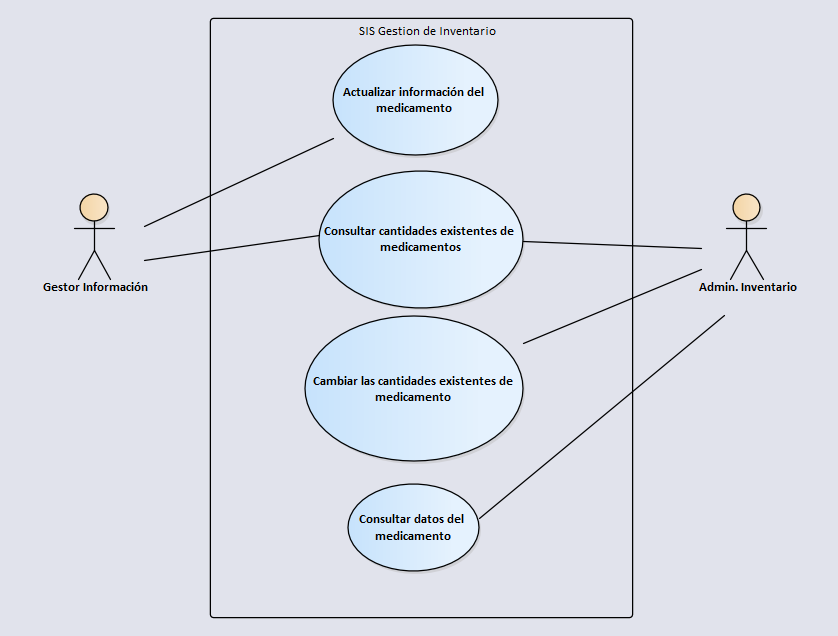
\includegraphics[width = 1.0\linewidth]{capitulo5/img/CasosUso.png}
\caption{Diagrama de Casos de Uso - Autor\'ia propia}
\end{figure}
\end{center}
\section{PIM: Modelo Independiente de la Plataforma}

\subsection{Diagramas Estructurales}

\subsubsection{Diagrama de Clases}

\begin{center}
    \begin{figure}[htb]
        \centering
        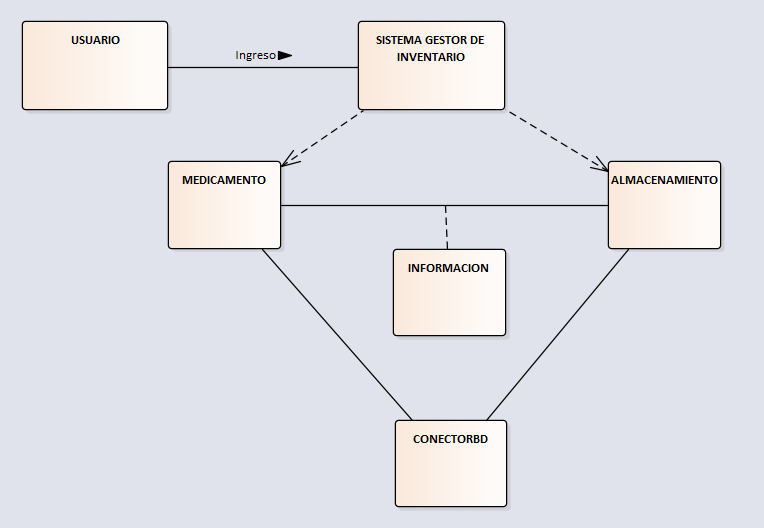
\includegraphics[width = 1.0\linewidth] {libro/capitulo5/img/Clases.PNG}
        \caption{Diagrama de Clases - Autor\'ia propia}
        \label{fig:my_label}
    \end{figure}
\end{center}

\subsection{ Diagramas de Comportamiento}
\subsubsection{ Diagrama de Estados}
Un diagrama de estados, en ocasiones conocido como diagrama de máquina de estados, es un tipo de diagrama de comportamiento en el Lenguaje Unificado de Modelado (UML) que muestra transiciones entre diversos objetos.
\newline
Cada diagrama de estados generalmente empieza con un círculo oscuro que indica el estado inicial y termina con un círculo de contorno blanco que denota el estado final. Estos representan principalmente estado y transiciones. Los estados se representan con rectángulos de esquinas redondeadas que se etiquetan con el nombre del estado. Las transiciones se marcan con flechas que fluyen de un estado a otro, mostrando cómo cambian los estados.


\begin{center}
    \begin{figure}[htb]
        \centering
        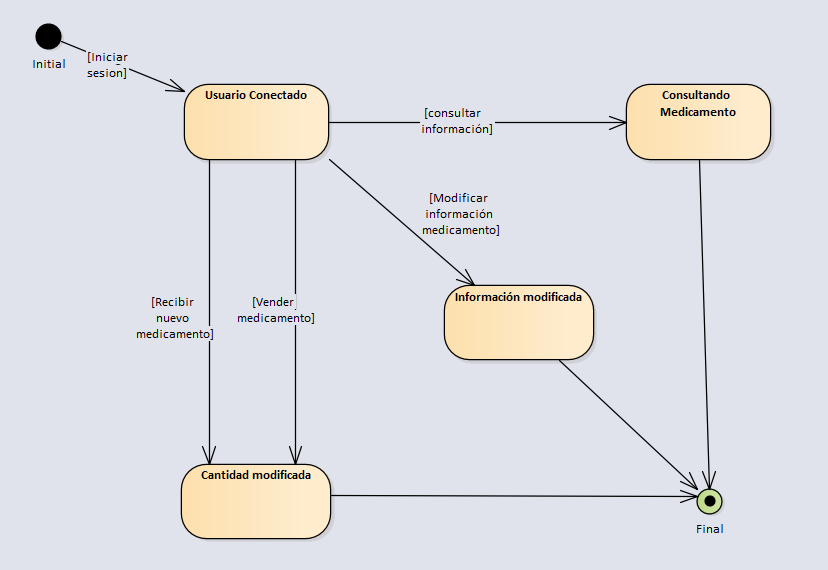
\includegraphics[width = 0.8\linewidth] {libro/capitulo5/img/Estados.png}
        \caption{Diagrama de Estados - Autor\'ia propia}
    \end{figure}
\end{center}
\subsubsection{ Diagrama de Actividades}

El Diagrama de Actividad es un diagrama de flujo del proceso multi-propósito que se usa para modelar el comportamiento del sistema. Los diagramas de actividad se pueden usar para modelar un Caso de Uso, o una clase, o un método complicado.
\newline
Un diagrama de actividad es parecido a un diagrama de flujo; la diferencia clave es que los diagramas de actividad pueden mostrar procesado paralelo (parallel processing). Esto es importante cuando se usan diagramas de actividad para modelar procesos 'bussiness' algunos de los cuales pueden actuar en paralelo, y para modelar varios hilos en los programas concurrentes.

\begin{center}
    \begin{figure}[htb]
        \centering
        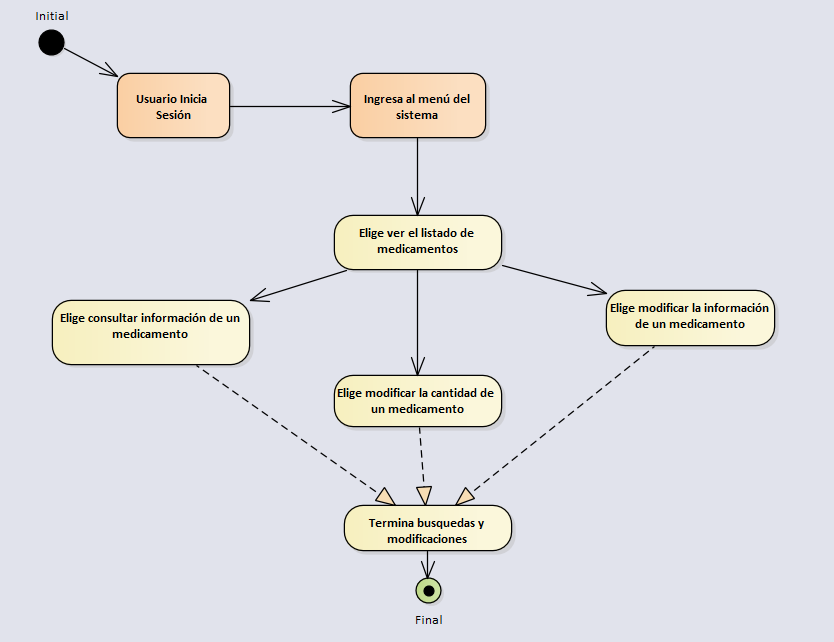
\includegraphics[width=1.0\linewidth] {capitulo5/img/Actividades.png}
        \caption{Diagrama de Actividades - Autor\'ia propia}
    \end{figure}
\end{center}
\newpage

\subsection{ Diagramas de Interacción}
\subsubsection{ Diagrama de Secuencia}

\begin{center}
    \begin{figure}[htb]
        \centering
        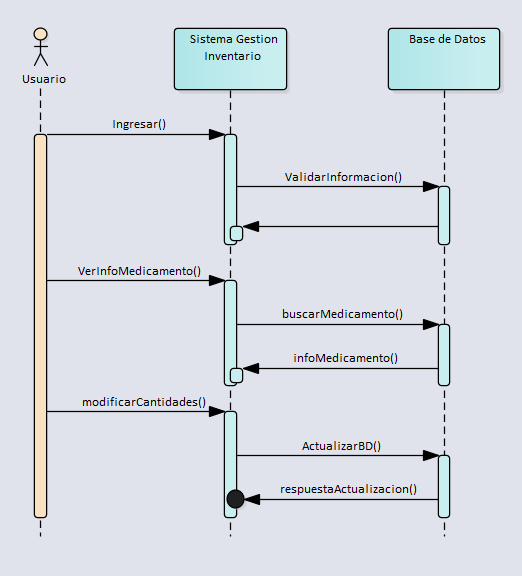
\includegraphics[width = 0.8\linewidth] {libro/capitulo5/img/Secuencia.PNG}
        \caption{Diagrama de Secuencia - Autor\'ia propia}
        \label{fig:my_label}
    \end{figure}
\end{center}

\newpage


\subsubsection{ Diagrama de Colaboración}
\begin{center}
    \begin{figure}[htb]
        \centering
        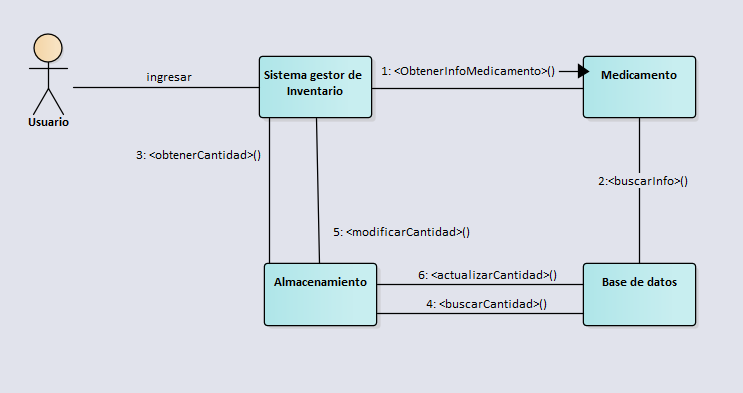
\includegraphics[width = 1.2\linewidth] {libro/capitulo5/img/Colaboracion.PNG}
        \caption{Diagrama de Colaboración - Autor\'ia propia}
        \label{fig:my_label}
    \end{figure}
\end{center}
\newpage

\subsection{ Diagramas de Implementación}
\subsubsection{ Diagrama de Componentes}
\begin{center}
    \begin{figure}[htb]
        \centering
        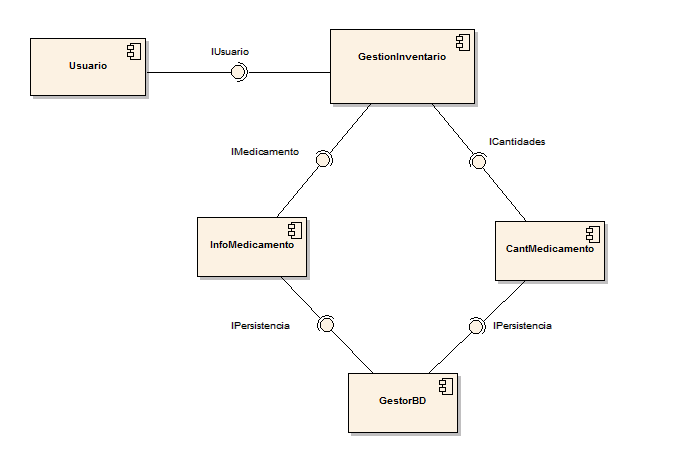
\includegraphics[width = 0.8\linewidth] {libro/capitulo5/img/Componentes.PNG}
        \caption{Diagrama de Componentes - Autor\'ia propia}
        \label{fig:my_label}
    \end{figure}
\end{center}
\subsubsection{Diagrama de Despliegue}

\begin{center}
    \begin{figure}[htb]
        \centering
        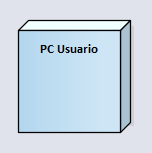
\includegraphics[width = 0.3\linewidth] {libro/capitulo5/img/Despliegue.PNG}
        \caption{Diagrama de Despliegue - Autor\'ia propia}
        \label{fig:my_label}
    \end{figure}
\end{center}

\section{PSM: Modelo Específico de Plataforma}

El aplicativo tratado en el presente documento ser\'a desarrollado en el lenguaje JAVA, con el IDE Eclipse y en la persistencia se usar\'a Postgress utilizando PGAdmin III para la gesti\'on de la base de datos.
